\chapter{LEVEL 1 @Problem 1 - 25}

\begin{chapquote}{Author's name, \textit{Source of this quote}}
	``This is a quote and I don't know who said this.''
\end{chapquote}

\section{Problem 001 - Multiples of 3 and 5}
\begin{prob}
If we list all the natural numbers below 10 that are multiples of 3 or 5, we get 3, 5, 6 and 9. The sum of these multiples is 23. Find the sum of all the multiples of 3 or 5 below 1000.
\end{prob}

\begin{sol}
Brute force is simple.
\code{code/001.c}
If using \emph{Including-Excluding Principle}, then denote $S_{k_1, k_2, \dots, k_n}$ as the sum of common multiples of $k_1, k_2,\dots,k_n$.
\begin{equation}
S = S_3 + S_5 - S_{3, 5} = S_3 + S_5 - S_{15}
\end{equation}
where $S_k$ can be calculated with $k\floor{\frac{n}{k}}( 1 + \floor{\frac{n}{k}})/2$.
\end{sol}

\section{Problem 002 - Even Fibonacci numbers}
\begin{prob}
Each new term in the Fibonacci sequence is generated by adding the previous two terms. By starting with 1 and 2, the first 10 terms will be:	
	$$1, 2, 3, 5, 8, 13, 21, 34, 55, 89, \dots$$
By considering the terms in the Fibonacci sequence whose values do not exceed four million, find the sum of the even-valued terms.
\end{prob}

\begin{sol}
It is simple to observe that the $F_{3k}$ is even. And we are looking for the summation $\sum_{k}^n F_{3k}$  over $k$ such that $F_{3n} \le N$. However, the following code computes the even numbers sequentially, time complexity $O(n)$, if there are $n$ elements before the loop ends.
\code{code/002.c}
To make this process faster, we can use the formula
\begin{equation}
F_n = \frac{1}{\sqrt{5}}\left(\left(\frac{1 + \sqrt{5}}{2}\right)^n - \left(\frac{1 - \sqrt{5}}{2}\right)^n\right)
\end{equation}
Which will be at cost of $O(\log n)$ complexity.
\end{sol}

\section{Problem 003 - Largest prime factor}
\begin{prob}
The prime factors of 13195 are 5, 7, 13 and 29.
What is the largest prime factor of the number 600851475143 ?
\end{prob}
\begin{sol}
Brute force is easy to implement, since the number overflows \texttt{int}, we use \texttt{long long int}. 
\code{code/003.c}
\end{sol}

\section{Problem 004 - Largest palindrome product}
\begin{prob}	
A palindromic number reads the same both ways. The largest palindrome made from the product of two 2-digit numbers is $9009 = 91 \times 99$.
Find the largest palindrome made from the product of two 3-digit numbers.
\end{prob}
\begin{sol}
The palindrome should be written as
\begin{equation}
\overline{abccba} = 100001 a + 10010 b + 1100 c = 11(9091 a + 910 b + 100 c)
\end{equation}
Now we can brute force the problem with one number divisible by 11.
\code{code/004.c}
\end{sol}

\section{Problem 005 - Smallest multiple}
\begin{prob}
2520 is the smallest number that can be divided by each of the numbers from 1 to 10 without any remainder.
What is the smallest positive number that is evenly divisible by all of the numbers from 1 to 20?
\end{prob}

\begin{sol}
\emph{LCM}(least common multiple) is as easy as \emph{GCD}(greatest common divider) by 
\begin{equation}
(a, b)[a, b] = ab
\end{equation}
We just iteratively calculate the \emph{LCM} from 1 to 20.
\code{code/005.c}
\end{sol}

\section{Problem 006 - Sum square difference}
\begin{prob}
The sum of the squares of the first ten natural numbers is,
$$1^2 + 2^2 + ... + 10^2 = 385$$
The square of the sum of the first ten natural numbers is,
$$(1 + 2 + ... + 10)^2 = 552 = 3025$$
Hence the difference between the sum of the squares of the first ten natural numbers and the square of the sum is $3025 - 385 = 2640$.
Find the difference between the sum of the squares of the first one hundred natural numbers and the square of the sum.
\end{prob}

\begin{sol}
Observe that
$$(\sum_{i = 1}^n i )^2 - \sum_{i = 1}^n i^2 = \frac{1}{4} n^2(n + 1)^2  - \frac{1}{6} n (n + 1)(2 n + 1)  = \frac{n(n + 1) (3 n ^2 - n - 2)}{12}$$
\end{sol}


\section{Problem 007 - 10001st prime}
\begin{prob}
By listing the first six prime numbers: 2, 3, 5, 7, 11, and 13, we can see that the 6th prime is 13.
What is the 10,001st prime number?
\end{prob}
\begin{sol}
We can use \href{http://en.wikipedia.org/wiki/Sieve_of_Eratosthenes}{\emph{Sieve algorithm}} to calculate the prime numbers below a given number $N$, and the estimated $p_n \sim n \log n$, thus $p_{10,001} \sim 115141$, we take $N = 200000$ for calculation. 
\code{code/007.c}
\end{sol}

\section{Problem 008 - Largest product in a series}
\begin{prob}
The four adjacent digits in the 1000-digit number that have the greatest product are $9 \times 9 \times 8 \times 9 = 5832$.

\begin{figure}[hb!]
\begin{center}
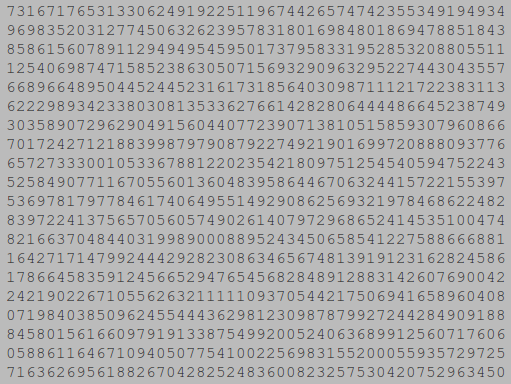
\includegraphics[scale = 0.52]{pic/008.png}
\end{center}
\end{figure}


\noindent Find the thirteen adjacent digits in the 1000-digit number that have the greatest product. What is the value of this product?
\end{prob}

\begin{sol}
Brute force.
\code{code/008.c}
\end{sol}

\section{Problem 009 - Special Pythagorean triplet}
\begin{prob}
A Pythagorean triplet is a set of three natural numbers, $a < b < c$, for which,
$$a^2 + b^2 = c^2$$
For example, $3^2 + 4^2 = 9 + 16 = 25 = 5^2$.

\noindent\\ There exists exactly one Pythagorean triplet for which $a + b + c = 1000$.
Find the product $abc$.
\end{prob}
\begin{sol}
It is known that Pythagorean triplet takes form of
$$(m^2 - n^2, 2mn, m^2 + n^2)$$
therefore, $2m^2 + 2mn = 1000$ only has one solution such that $m > n$.
\begin{eqnarray}
m^2 + m < m(m + n) = 500 < 2 m ^2
\end{eqnarray}
then $23 > m > 15$, there is only one solution $m = 20, n = 5$.
\end{sol}


\section{Problem 010 - Summation of primes}
\begin{prob}
The sum of the primes below 10 is 2 + 3 + 5 + 7 = 17.
Find the sum of all the primes below two million.
\end{prob}
\begin{sol}
Brute force. Use sieve algorithm to find all the prime numbers, and sum them up.
\code{code/010.c}
\end{sol}
\newpage
\section{Problem 011 - Largest product in a grid}
\begin{prob}
In the $20\times20$ grid below, four numbers along a diagonal line have been marked in red.
\begin{figure}[htb]
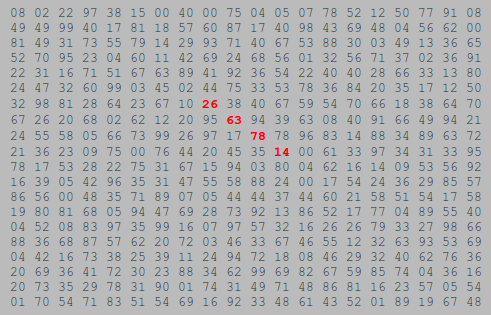
\includegraphics[scale = 0.73]{pic/010.png}
\end{figure}
\noindent\\The product of these numbers is $26 \times 63 \times 78 \times 14 = 1788696$.

\noindent\\What is the greatest product of four adjacent numbers in the same direction (up, down, left, right, or diagonally) in the $20 \times 20$ grid?
\end{prob}

\begin{sol}
Brute force.
\code{code/011.c}
\end{sol}

\newpage
\section{Problem 012 - Highly divisible triangular number}
\begin{prob}
\begin{figure}[htb!]
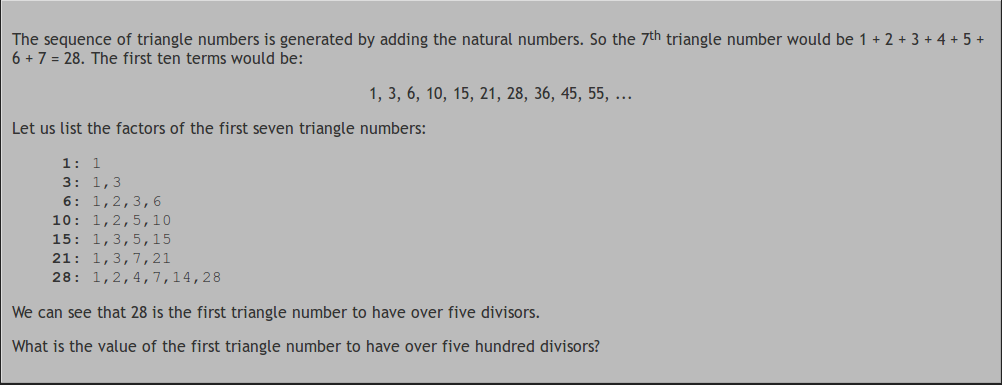
\includegraphics[scale = 0.4]{pic/012.png}
\end{figure}
\end{prob}
\begin{sol}
Brute force.
\code{code/012.c}
\end{sol}

\section{Problem 013 - Large sum}
\begin{prob}
Work out the first ten digits of the sum of the following one-hundred 50-digit numbers. \href{https://projecteuler.net/problem=13}{See data here.}
\end{prob}
\begin{sol}
The quick way is to use double type to save the numbers as $\overline{a.bcdefgh\dots}$, though machine error will only give limited accuracy around $10^{-15}$, but it is more than enough, when converting back into integer, be careful of possible overflow.
\code{code/013.c}
\end{sol}
\newpage
\section{Problem 014 - Longest Collatz sequence}
\begin{prob}
	\begin{figure}[htb!]
		\begin{center}
			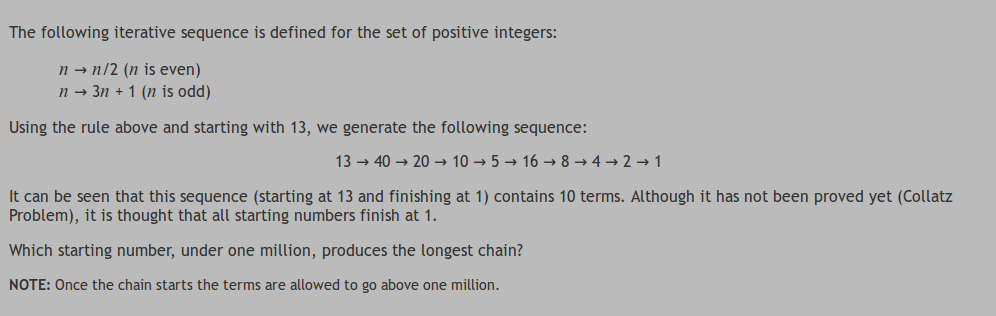
\includegraphics[scale = 0.4]{pic/014.png}
		\end{center}
	\end{figure}
\end{prob}

\begin{sol}
Brute force. Calculate the length of sequence for each start.
\code{code/014.c}
\end{sol}
\newpage
\section{Problem 015 - Lattice paths}
\begin{prob}
	\begin{figure}[htb!]
		\begin{center}
			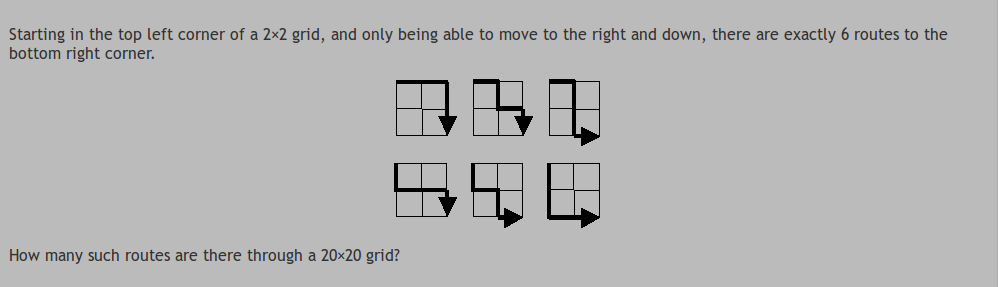
\includegraphics[scale = 0.4]{pic/015.png}
		\end{center}
	\end{figure}
\end{prob}

\begin{sol}
Suppose $f(m,n)$ represents the number of path for lattice $m \ times n$, then it is easy to observe:
$$f(m, n) = f(m - 1, n) + f(m, n - 1)$$
and $f(m, 0) = 1$, $f(0, n) = 1$. 
On the other hand, we only have $m$ steps moving right, and $n$ steps down. Thus it is equivalent to say we choose $m$ steps out of $(m + n)$ steps to move right, the rest are for moving down, which gives ${m + n}\choose m $.

\noindent \\For this problem 
$${40 \choose 20} = \frac{40!}{20! 20!} = \frac{40 \times 39 \times\dots 21}{20 \times 19\times \dots 1}$$

\noindent \\Using \texttt{long long} type should be enough to calculate.
\end{sol}
\section{Problem 016 - Power digit sum}
\begin{prob}
\begin{figure}[htb!]
	\begin{center}
	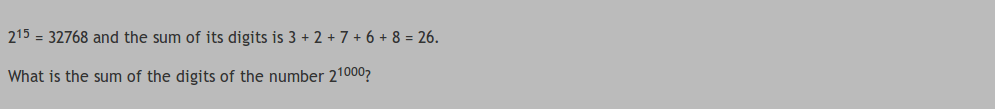
\includegraphics[scale = 0.4]{pic/016.png}
	\end{center}
\end{figure}
\end{prob}

\begin{sol}
Brute force using \texttt{Python} is extremely easy, since it can display all digits (around 300) of $2^{1000}$. Using \texttt{string} to represent the number is also fast.
\end{sol}
\section{Problem 017}
\begin{prob}
\end{prob}
\section{Problem 018}
\begin{prob}
\end{prob}
\section{Problem 019}
\begin{prob}
\end{prob}
\section{Problem 020}
\begin{prob}
\end{prob}
\section{Problem 021}
\begin{prob}
\end{prob}
\section{Problem 022}
\begin{prob}
\end{prob}
\section{Problem 023}
\begin{prob}
\end{prob}
\section{Problem 024}
\begin{prob}
\end{prob}
\section{Problem 025}
\begin{prob}
\end{prob}